\section{Distributed Worlds and Playable Cities}
\label{sec:distributed-playable}

v2 introduces a hub-and-node protocol that lets a single open world be
partitioned across many machines.  The hub is the dashboard server; each
node is a worker machine that runs the simulation for a subset of the
world's residents with the node's own model key.  Players continue to
interact through a browser; the hub routes their interventions to the
node that owns the relevant resident.  Figure~\ref{fig:hub-node} depicts
the topology.

\begin{figure}[t]
  \centering
  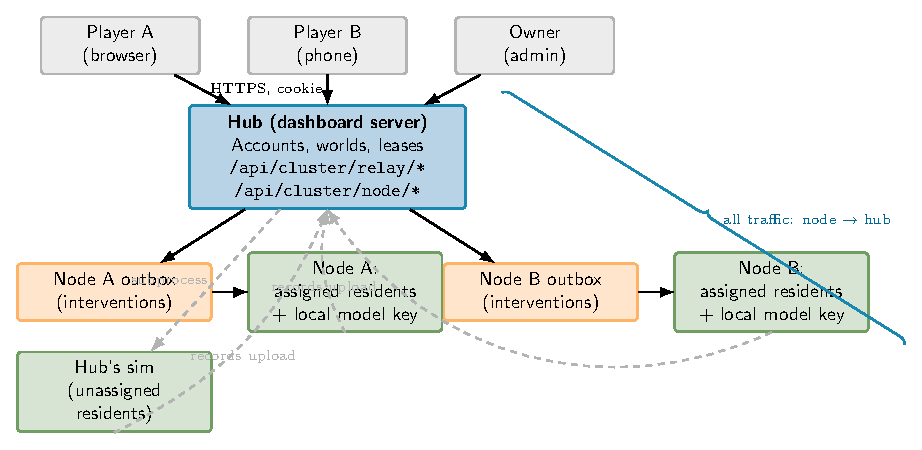
\includegraphics[width=\linewidth]{hub_node.pdf}
  \caption{Distributed playable topology.  The hub is the dashboard server;
  it owns accounts, the world metadata, the per-node outbox, the per-world
  relay, and the per-tenant Recorder merge.  Each node runs the simulation
  for its assigned residents, polls interventions, and uploads Recorder
  rows.  All cross-machine traffic is node-to-hub; the hub never opens
  inbound ports to a node.}
  \label{fig:hub-node}
\end{figure}

\subsection{Topology and threat model}

The topology is asymmetric on purpose: all traffic is node $\to$ hub.
Nodes can sit behind NAT, behind phone hotspots, or in a firewall; they
need only an outbound HTTPS connection to the hub.  This is a deliberate
trade-off: the protocol does not need a clock-synchronization primitive
because the hub does not advance simulation time.  Each node runs the
simulation locally; the hub merges per-node Recorder rows and routes
interventions.  No transactional consistency is offered; the protocol
is best-effort and tolerates brief disconnection.

The hub is the dashboard server; this means one port, one reverse proxy,
one TLS certificate for a public deployment.  The v1 standalone relay
(\texttt{distributed\_comm\_server}) is retained for OpenClaw-style
deployments, but in v2 it is no longer required: the dashboard server
embeds the relay as an in-process \texttt{DistributedRelayBackend}, one
per world.  The hub itself is also a node, identified as
\texttt{node\_id = hub}; it runs the simulation for residents that have
not been assigned to any external node, so that the world has at least
one heartbeat even when every external node is offline.

\subsection{Node lifecycle}

A node is added by the world's owner through the dashboard.  The owner
fills in a name (e.g., ``Lab 302 seat 7'') and a list of residents that
the node should run (either a list of ids or ``rebalance N'').  The hub
issues a one-time token of the form
$\texttt{world\_id}.\texttt{node\_id}.\texttt{secret}$, shows it once,
and stores the SHA-256 of the secret.  The secret is therefore a bearer
token; its revocation is immediate, and a revoked node receives a 401 on
its next heartbeat and stops the simulation.

The node process is a single Python command:

\begin{verbatim}
  python -m gaworld.cluster join <hub-url> --token <token>
\end{verbatim}

The node begins by sending a heartbeat.  The hub responds with
``world is running; new run id is \texttt{R}; please download the
world bundle''.  The node downloads a zip containing the world's
configuration, the seed \texttt{agents.csv} and \texttt{profiles.md},
and the city bundle.  It then launches the simulation subprocess with
\texttt{GAWORLD\_CONFIG\_OVERRIDES} carrying the world's configuration,
the per-node paths, the assigned residents, and the relay's URL and
token.  The simulation code does not change between local and remote
modes; only the override environment differs.

While the simulation runs, the node polls interventions every second,
enqueues them locally through the standard \texttt{kernel/remote}
interface, and the simulation drains the queue at the next tick as in v1.
The node also reads the per-table \texttt{records/*.jsonl} files every
second and uploads new rows to the hub, which appends them to the
world's merged Recorder with a \texttt{\_node} tag on each row.  When
the hub says ``stop'', the node terminates the subprocess; when the
subprocess exits on its own, the node reports that status in the next
heartbeat.  When the network is offline, the node keeps running and
back-fills records when the connection returns; when the simulation's
tick-sync timeout expires, the node advances without waiting.

\subsection{Player action routing}

A player intervention (\texttt{player\_claim}, \texttt{player\_act},
\texttt{player\_say}, or \texttt{player\_release}) is received by the
hub through the dashboard's \texttt{play} API.  The hub resolves the
intervention's target resident and routes it:

\begin{itemize}[leftmargin=*]
  \item If the resident is on the hub, the intervention is appended to
  the hub's local queue (as in v1).
  \item If the resident is on a remote node, the intervention is
  appended to that node's outbox; the next time the node polls
  (\textless 1 s in the v2 implementation), the intervention enters its
  local queue and is consumed at the next tick.
  \item For \texttt{player\_say}, the speaker and the listener may be on
  different nodes.  The speaker's node records ``you said X to Y'' as
  a local action; the listener's node receives a \texttt{player\_hear}
  intervention that adds ``Y said: X'' to the listener's next
  perception.
\end{itemize}

Player leases remain on the hub (\texttt{play\_api.\_CLAIMS}).  A
node's simulation does not need to know that the player exists; the
lease is the hub's bookkeeping, refreshed every 30 s.  If a node
disconnects, the lease remains valid on the hub and the player can
continue to be served; when the node reconnects, it re-registers any
active claims so the simulation can keep them consistent.

\subsection{Clock synchronization}

The hub and each node maintain a \emph{logical} clock that is updated
whenever a Recorder row arrives.  The simulation is allowed to advance
its own clock without coordination, so the protocol is not a
conservative-synchronization protocol: it tolerates drift.  Each node
periodically reports its clock to the hub, and the hub publishes a
\emph{median} clock that downstream code can use to align downstream
consumers (the visualizer, the Auditor UI, the intervention display).
The current implementation does not implement rollback or
deterministic-replay, and the protocol does not promise a
tighter-than-seconds clock alignment.  This is the trade-off that
makes the system operable behind NATs and is the reason the protocol
is best-effort.

\subsection{Security and access control}

Node tokens grant access to the per-world \texttt{/api/cluster/node/*}
and \texttt{/api/cluster/relay/*} endpoints; they do not grant access
to the dashboard, the account store, or to any other world.  Bearer
authentication is required for every request; the node id is bound to
the secret, and the secret is checked against a SHA-256 hash.  The hub
emits a structured audit row on every node request, including
``heartbeat'', ``bundle-download'', ``intervention-poll'',
``records-upload'', ``sync'', and ``denied''.  A revoked node receives
401 on its next request and stops the simulation.  When a node's
\texttt{node\_id} is reused after a restart, the new secret replaces
the old hash; the old secret is invalidated atomically.

\subsection{Deployment profiles}

A v2 deployment can be configured in three profiles:

\begin{itemize}[leftmargin=*]
  \item \textbf{Single tenant, single process} (v1-equivalent): accounts
  are off, the relay is in-process, and the only node is the hub.  This
  is the default for local research and for the bundled benchmarks.
  \item \textbf{Multi-tenant, single process}: accounts are on, the
  relay is in-process, and the only node is the hub.  This is the
  default for a classroom or workshop.
  \item \textbf{Multi-tenant, multi-node}: accounts are on, the relay
  is in-process, and one or more external nodes are connected.  This
  is the default for cross-machine deployments (a school lab, a
  cross-campus collaboration, a multi-region test).
\end{itemize}

The same code path runs in all three profiles; the differences are
configuration, not code.  A multi-node deployment does not promise
horizontal scalability, throughput improvement, or fault tolerance; it
promises the ability to assign residents to machines that have their
own model keys, and the ability to keep a world alive when one node
disconnects.
